% Options for packages loaded elsewhere
\PassOptionsToPackage{unicode}{hyperref}
\PassOptionsToPackage{hyphens}{url}
\PassOptionsToPackage{dvipsnames,svgnames,x11names}{xcolor}
%
\documentclass[
]{book}
\usepackage{amsmath,amssymb}
\usepackage{iftex}
\ifPDFTeX
  \usepackage[T1]{fontenc}
  \usepackage[utf8]{inputenc}
  \usepackage{textcomp} % provide euro and other symbols
\else % if luatex or xetex
  \usepackage{unicode-math} % this also loads fontspec
  \defaultfontfeatures{Scale=MatchLowercase}
  \defaultfontfeatures[\rmfamily]{Ligatures=TeX,Scale=1}
\fi
\usepackage{lmodern}
\ifPDFTeX\else
  % xetex/luatex font selection
\fi
% Use upquote if available, for straight quotes in verbatim environments
\IfFileExists{upquote.sty}{\usepackage{upquote}}{}
\IfFileExists{microtype.sty}{% use microtype if available
  \usepackage[]{microtype}
  \UseMicrotypeSet[protrusion]{basicmath} % disable protrusion for tt fonts
}{}
\makeatletter
\@ifundefined{KOMAClassName}{% if non-KOMA class
  \IfFileExists{parskip.sty}{%
    \usepackage{parskip}
  }{% else
    \setlength{\parindent}{0pt}
    \setlength{\parskip}{6pt plus 2pt minus 1pt}}
}{% if KOMA class
  \KOMAoptions{parskip=half}}
\makeatother
\usepackage{xcolor}
\usepackage{color}
\usepackage{fancyvrb}
\newcommand{\VerbBar}{|}
\newcommand{\VERB}{\Verb[commandchars=\\\{\}]}
\DefineVerbatimEnvironment{Highlighting}{Verbatim}{commandchars=\\\{\}}
% Add ',fontsize=\small' for more characters per line
\usepackage{framed}
\definecolor{shadecolor}{RGB}{248,248,248}
\newenvironment{Shaded}{\begin{snugshade}}{\end{snugshade}}
\newcommand{\AlertTok}[1]{\textcolor[rgb]{0.94,0.16,0.16}{#1}}
\newcommand{\AnnotationTok}[1]{\textcolor[rgb]{0.56,0.35,0.01}{\textbf{\textit{#1}}}}
\newcommand{\AttributeTok}[1]{\textcolor[rgb]{0.13,0.29,0.53}{#1}}
\newcommand{\BaseNTok}[1]{\textcolor[rgb]{0.00,0.00,0.81}{#1}}
\newcommand{\BuiltInTok}[1]{#1}
\newcommand{\CharTok}[1]{\textcolor[rgb]{0.31,0.60,0.02}{#1}}
\newcommand{\CommentTok}[1]{\textcolor[rgb]{0.56,0.35,0.01}{\textit{#1}}}
\newcommand{\CommentVarTok}[1]{\textcolor[rgb]{0.56,0.35,0.01}{\textbf{\textit{#1}}}}
\newcommand{\ConstantTok}[1]{\textcolor[rgb]{0.56,0.35,0.01}{#1}}
\newcommand{\ControlFlowTok}[1]{\textcolor[rgb]{0.13,0.29,0.53}{\textbf{#1}}}
\newcommand{\DataTypeTok}[1]{\textcolor[rgb]{0.13,0.29,0.53}{#1}}
\newcommand{\DecValTok}[1]{\textcolor[rgb]{0.00,0.00,0.81}{#1}}
\newcommand{\DocumentationTok}[1]{\textcolor[rgb]{0.56,0.35,0.01}{\textbf{\textit{#1}}}}
\newcommand{\ErrorTok}[1]{\textcolor[rgb]{0.64,0.00,0.00}{\textbf{#1}}}
\newcommand{\ExtensionTok}[1]{#1}
\newcommand{\FloatTok}[1]{\textcolor[rgb]{0.00,0.00,0.81}{#1}}
\newcommand{\FunctionTok}[1]{\textcolor[rgb]{0.13,0.29,0.53}{\textbf{#1}}}
\newcommand{\ImportTok}[1]{#1}
\newcommand{\InformationTok}[1]{\textcolor[rgb]{0.56,0.35,0.01}{\textbf{\textit{#1}}}}
\newcommand{\KeywordTok}[1]{\textcolor[rgb]{0.13,0.29,0.53}{\textbf{#1}}}
\newcommand{\NormalTok}[1]{#1}
\newcommand{\OperatorTok}[1]{\textcolor[rgb]{0.81,0.36,0.00}{\textbf{#1}}}
\newcommand{\OtherTok}[1]{\textcolor[rgb]{0.56,0.35,0.01}{#1}}
\newcommand{\PreprocessorTok}[1]{\textcolor[rgb]{0.56,0.35,0.01}{\textit{#1}}}
\newcommand{\RegionMarkerTok}[1]{#1}
\newcommand{\SpecialCharTok}[1]{\textcolor[rgb]{0.81,0.36,0.00}{\textbf{#1}}}
\newcommand{\SpecialStringTok}[1]{\textcolor[rgb]{0.31,0.60,0.02}{#1}}
\newcommand{\StringTok}[1]{\textcolor[rgb]{0.31,0.60,0.02}{#1}}
\newcommand{\VariableTok}[1]{\textcolor[rgb]{0.00,0.00,0.00}{#1}}
\newcommand{\VerbatimStringTok}[1]{\textcolor[rgb]{0.31,0.60,0.02}{#1}}
\newcommand{\WarningTok}[1]{\textcolor[rgb]{0.56,0.35,0.01}{\textbf{\textit{#1}}}}
\usepackage{longtable,booktabs,array}
\usepackage{calc} % for calculating minipage widths
% Correct order of tables after \paragraph or \subparagraph
\usepackage{etoolbox}
\makeatletter
\patchcmd\longtable{\par}{\if@noskipsec\mbox{}\fi\par}{}{}
\makeatother
% Allow footnotes in longtable head/foot
\IfFileExists{footnotehyper.sty}{\usepackage{footnotehyper}}{\usepackage{footnote}}
\makesavenoteenv{longtable}
\usepackage{graphicx}
\makeatletter
\def\maxwidth{\ifdim\Gin@nat@width>\linewidth\linewidth\else\Gin@nat@width\fi}
\def\maxheight{\ifdim\Gin@nat@height>\textheight\textheight\else\Gin@nat@height\fi}
\makeatother
% Scale images if necessary, so that they will not overflow the page
% margins by default, and it is still possible to overwrite the defaults
% using explicit options in \includegraphics[width, height, ...]{}
\setkeys{Gin}{width=\maxwidth,height=\maxheight,keepaspectratio}
% Set default figure placement to htbp
\makeatletter
\def\fps@figure{htbp}
\makeatother
\setlength{\emergencystretch}{3em} % prevent overfull lines
\providecommand{\tightlist}{%
  \setlength{\itemsep}{0pt}\setlength{\parskip}{0pt}}
\setcounter{secnumdepth}{5}
\usepackage{booktabs}
\usepackage{booktabs}
\usepackage{longtable}
\usepackage{array}
\usepackage{multirow}
\usepackage{wrapfig}
\usepackage{float}
\usepackage{colortbl}
\usepackage{pdflscape}
\usepackage{tabu}
\usepackage{threeparttable}
\usepackage{threeparttablex}
\usepackage[normalem]{ulem}
\usepackage{makecell}
\usepackage{xcolor}
\ifLuaTeX
  \usepackage{selnolig}  % disable illegal ligatures
\fi
\usepackage[]{natbib}
\bibliographystyle{plainnat}
\IfFileExists{bookmark.sty}{\usepackage{bookmark}}{\usepackage{hyperref}}
\IfFileExists{xurl.sty}{\usepackage{xurl}}{} % add URL line breaks if available
\urlstyle{same}
\hypersetup{
  pdftitle={R Basic Course},
  pdfauthor={Mardones, Mauricio. \& Zúñiga, María José.},
  colorlinks=true,
  linkcolor={blue},
  filecolor={Maroon},
  citecolor={Blue},
  urlcolor={Blue},
  pdfcreator={LaTeX via pandoc}}

\title{R Basic Course}
\author{Mardones, Mauricio. \& Zúñiga, María José.}
\date{2025-02-07}

\begin{document}
\maketitle

{
\hypersetup{linkcolor=}
\setcounter{tocdepth}{1}
\tableofcontents
}
\hypertarget{about-course_r}{%
\chapter*{About Course\_R}\label{about-course_r}}
\addcontentsline{toc}{chapter}{About Course\_R}

Description and educational material for introductory course on R, descriptive statistics, and visualizations with applications in fisheries.

This course has these sections;

\begin{itemize}
\item
  \begin{enumerate}
  \def\labelenumi{\arabic{enumi}.}
  \tightlist
  \item
    \textbf{useR}. Intro to R and basic features.
  \end{enumerate}
\item
  \begin{enumerate}
  \def\labelenumi{\arabic{enumi}.}
  \setcounter{enumi}{1}
  \tightlist
  \item
    \textbf{Exploratory Data Analysis}. Basic concepts for data exploration.
  \end{enumerate}
\item
  \begin{enumerate}
  \def\labelenumi{\arabic{enumi}.}
  \setcounter{enumi}{2}
  \tightlist
  \item
    \textbf{Descriptive Statistics}. Essential statistical calculations.
  \end{enumerate}
\item
  \begin{enumerate}
  \def\labelenumi{\arabic{enumi}.}
  \setcounter{enumi}{3}
  \tightlist
  \item
    \textbf{Visualization}. Graphics and Maps using modern packages
  \end{enumerate}
\item
  \begin{enumerate}
  \def\labelenumi{\arabic{enumi}.}
  \setcounter{enumi}{4}
  \tightlist
  \item
    \textbf{Efficient code}. Organization strategies.\\
  \end{enumerate}
\item
  \begin{enumerate}
  \def\labelenumi{\arabic{enumi}.}
  \setcounter{enumi}{5}
  \tightlist
  \item
    \textbf{Automatization and sharing} Report generation and result sharing.\\
  \end{enumerate}
\item
  \begin{enumerate}
  \def\labelenumi{\arabic{enumi}.}
  \setcounter{enumi}{6}
  \tightlist
  \item
    \textbf{Management of Bibliographic} sources and additional materials.
  \end{enumerate}
\end{itemize}

All codes and used in this course can be founded in this repository with the structure to do this Ebook
\href{https://github.com/MauroMardones/Course_R_Statistics}{Repo R Course}

\hypertarget{user.-intro-to-r-and-basic-features}{%
\chapter{\texorpdfstring{\textbf{useR}. Intro to R and basic features}{useR. Intro to R and basic features}}\label{user.-intro-to-r-and-basic-features}}

\hypertarget{welcome-r-user}{%
\section{Welcome R user}\label{welcome-r-user}}

\begin{itemize}
\tightlist
\item
  \textbf{R} is a programming language designed for:

  \begin{itemize}
  \tightlist
  \item
    Statistical computing
  \item
    Data analysis
  \item
    Visualization
  \end{itemize}
\end{itemize}

\begin{center}
\includegraphics[width=0.5\linewidth]{images/rpages} \end{center}

\href{https://www.r-project.org}{Download R}

\begin{center}
\includegraphics[width=0.5\linewidth]{images/rpages} \end{center}

\href{https://posit.co/download/rstudio-desktop/}{Download Rstudio}

\hypertarget{why-learn-r}{%
\section{¿Why learn R?}\label{why-learn-r}}

\begin{itemize}
\tightlist
\item
  Open source and free\\
\item
  big community\\
\item
  \textasciitilde{} 13.000 packages\\
\item
  Reproducible science
\end{itemize}

is just this

\begin{center}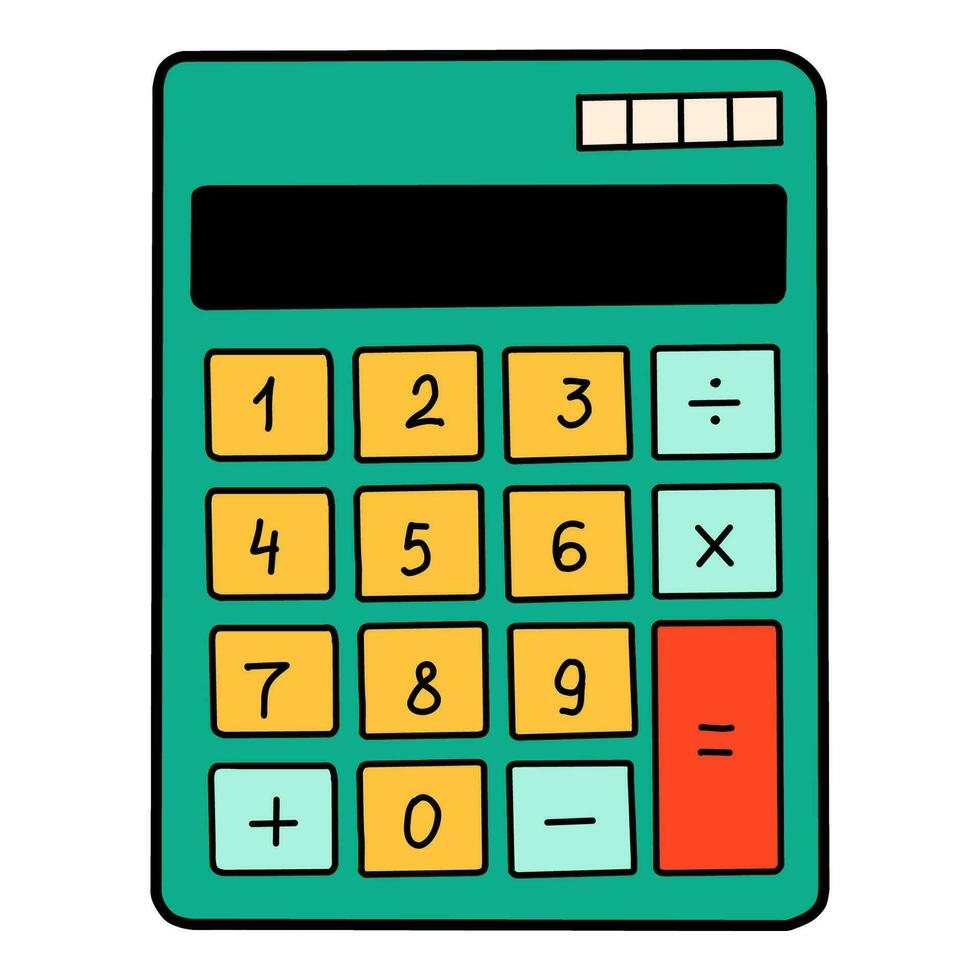
\includegraphics[width=0.9\linewidth]{images/calc} \end{center}

but\ldots{}

\hypertarget{origin-of-r}{%
\section{Origin of R}\label{origin-of-r}}

Seminal paper or R! \href{http://www.aliquote.org/cours/2012_biomed/biblio/Ihaka1996.pdf}{here} (Fig. \ref{fig:semi}).

\begin{figure}

{\centering 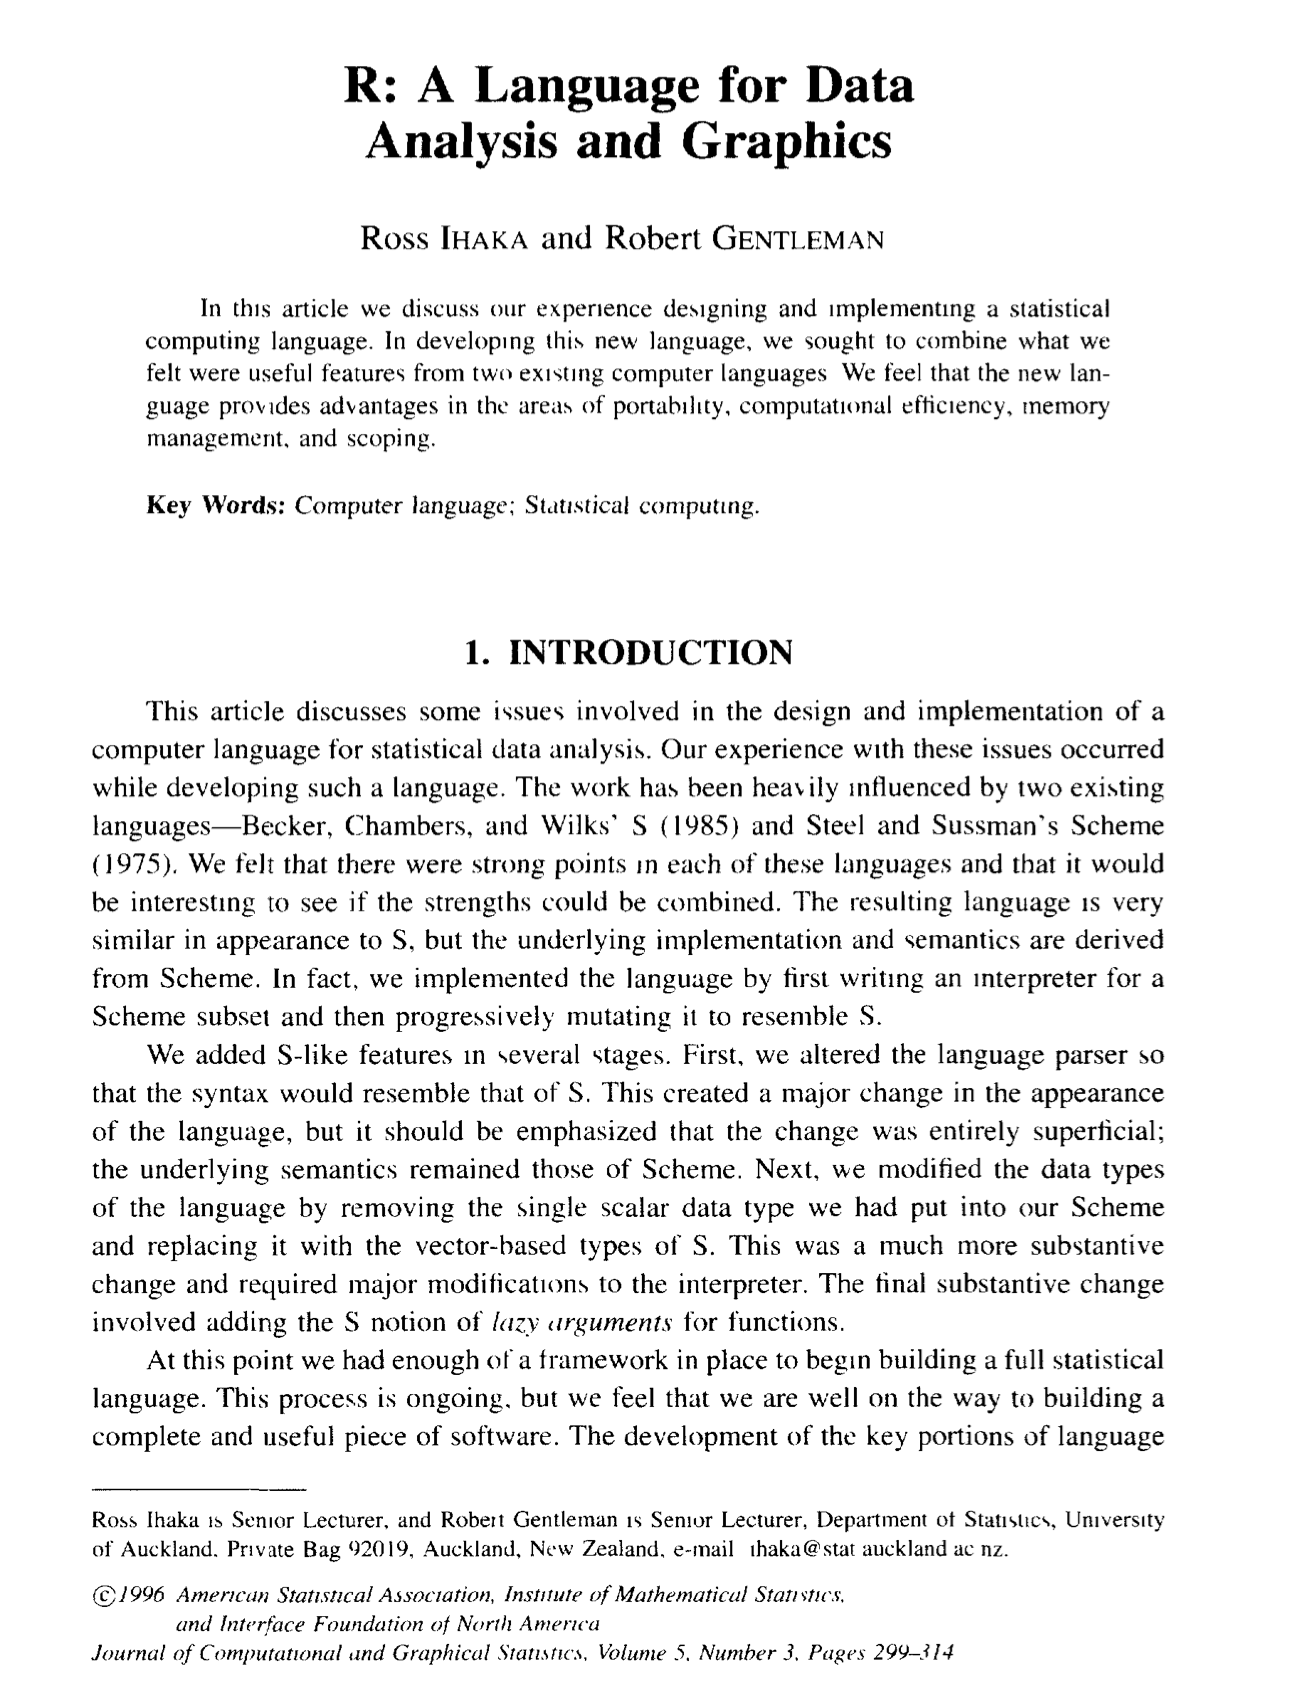
\includegraphics[width=0.9\linewidth]{images/papeR} 

}

\caption{Seminal Paper of R}\label{fig:semi}
\end{figure}

\hypertarget{getting-started}{%
\section{Getting Started}\label{getting-started}}

\begin{enumerate}
\def\labelenumi{\arabic{enumi}.}
\tightlist
\item
  Install R from \href{https://cran.r-project.org}{CRAN}
\item
  Install RStudio (optional, but highly recommended)
\item
  Write your first R command:
\end{enumerate}

\begin{Shaded}
\begin{Highlighting}[]
\FunctionTok{print}\NormalTok{(}\StringTok{"Hello, world!"}\NormalTok{)}
\end{Highlighting}
\end{Shaded}

\begin{verbatim}
## [1] "Hello, world!"
\end{verbatim}

\hypertarget{basic-data-types}{%
\section{Basic Data Types}\label{basic-data-types}}

\begin{itemize}
\tightlist
\item
  \textbf{Numeric:} Numbers (e.g., \texttt{3.14}, \texttt{42})
\item
  \textbf{Character:} Text strings (e.g., \texttt{"fish"})
\item
  \textbf{Logical:} \texttt{TRUE} or \texttt{FALSE}
\item
  \textbf{Factor:} Categorical variables
\end{itemize}

\hypertarget{vectors}{%
\section{Vectors}\label{vectors}}

\begin{itemize}
\tightlist
\item
  R's most fundamental data structure:
\end{itemize}

\begin{Shaded}
\begin{Highlighting}[]
\NormalTok{numbers }\OtherTok{\textless{}{-}} \FunctionTok{c}\NormalTok{(}\DecValTok{1}\NormalTok{, }\DecValTok{2}\NormalTok{, }\DecValTok{3}\NormalTok{, }\DecValTok{4}\NormalTok{)}
\NormalTok{letters }\OtherTok{\textless{}{-}} \FunctionTok{c}\NormalTok{(}\StringTok{"a"}\NormalTok{, }\StringTok{"b"}\NormalTok{, }\StringTok{"c"}\NormalTok{)}
\end{Highlighting}
\end{Shaded}

\begin{itemize}
\tightlist
\item
  Operations are vectorized:
\end{itemize}

\begin{Shaded}
\begin{Highlighting}[]
\NormalTok{numbers }\SpecialCharTok{*} \DecValTok{2}
\end{Highlighting}
\end{Shaded}

\begin{verbatim}
## [1] 2 4 6 8
\end{verbatim}

\hypertarget{data-frames}{%
\section{Data Frames}\label{data-frames}}

\begin{itemize}
\tightlist
\item
  Table-like structures:
\end{itemize}

\begin{Shaded}
\begin{Highlighting}[]
\NormalTok{df }\OtherTok{\textless{}{-}} \FunctionTok{data.frame}\NormalTok{(}\AttributeTok{Name =} \FunctionTok{c}\NormalTok{(}\StringTok{"John"}\NormalTok{, }\StringTok{"Jane"}\NormalTok{),}
    \AttributeTok{Age =} \FunctionTok{c}\NormalTok{(}\DecValTok{25}\NormalTok{, }\DecValTok{30}\NormalTok{))}
\end{Highlighting}
\end{Shaded}

\begin{itemize}
\tightlist
\item
  Inspect the structure:
\end{itemize}

\begin{Shaded}
\begin{Highlighting}[]
\FunctionTok{head}\NormalTok{(df)}
\end{Highlighting}
\end{Shaded}

\begin{verbatim}
##   Name Age
## 1 John  25
## 2 Jane  30
\end{verbatim}

\hypertarget{visualization}{%
\section{Visualization}\label{visualization}}

\begin{itemize}
\tightlist
\item
  Example base plot:
\end{itemize}

Data used

\begin{Shaded}
\begin{Highlighting}[]
\FunctionTok{kbl}\NormalTok{(}\FunctionTok{head}\NormalTok{(iris))}
\end{Highlighting}
\end{Shaded}

\begin{tabular}[t]{r|r|r|r|l}
\hline
Sepal.Length & Sepal.Width & Petal.Length & Petal.Width & Species\\
\hline
5.1 & 3.5 & 1.4 & 0.2 & setosa\\
\hline
4.9 & 3.0 & 1.4 & 0.2 & setosa\\
\hline
4.7 & 3.2 & 1.3 & 0.2 & setosa\\
\hline
4.6 & 3.1 & 1.5 & 0.2 & setosa\\
\hline
5.0 & 3.6 & 1.4 & 0.2 & setosa\\
\hline
5.4 & 3.9 & 1.7 & 0.4 & setosa\\
\hline
\end{tabular}

\begin{Shaded}
\begin{Highlighting}[]
\NormalTok{plottex }\OtherTok{\textless{}{-}} \FunctionTok{ggplot}\NormalTok{(iris, }\FunctionTok{aes}\NormalTok{(}\AttributeTok{x =}\NormalTok{ Sepal.Length,}
    \AttributeTok{y =}\NormalTok{ Species)) }\SpecialCharTok{+} \FunctionTok{geom\_bar}\NormalTok{(}\AttributeTok{stat =} \StringTok{"identity"}\NormalTok{)}
\NormalTok{plottex}
\end{Highlighting}
\end{Shaded}

\begin{center}
\includegraphics[width=0.6\linewidth]{_main_files/figure-latex/unnamed-chunk-12-1} \end{center}

\begin{Shaded}
\begin{Highlighting}[]
\NormalTok{plottex }\OtherTok{\textless{}{-}} \FunctionTok{ggplot}\NormalTok{(iris, }\FunctionTok{aes}\NormalTok{(}\AttributeTok{x =}\NormalTok{ Sepal.Length,}
    \AttributeTok{y =}\NormalTok{ Species)) }\SpecialCharTok{+} \FunctionTok{geom\_bar}\NormalTok{(}\AttributeTok{stat =} \StringTok{"identity"}\NormalTok{) }\SpecialCharTok{+}
    \FunctionTok{theme\_minimal}\NormalTok{()}
\NormalTok{plottex}
\end{Highlighting}
\end{Shaded}

\begin{center}
\includegraphics[width=0.6\linewidth]{_main_files/figure-latex/unnamed-chunk-13-1} \end{center}

\begin{Shaded}
\begin{Highlighting}[]
\NormalTok{plottex }\OtherTok{\textless{}{-}} \FunctionTok{ggplot}\NormalTok{(iris, }\FunctionTok{aes}\NormalTok{(}\AttributeTok{x =}\NormalTok{ Sepal.Length,}
    \AttributeTok{y =}\NormalTok{ Species)) }\SpecialCharTok{+} \FunctionTok{geom\_bar}\NormalTok{(}\AttributeTok{stat =} \StringTok{"identity"}\NormalTok{) }\SpecialCharTok{+}
    \FunctionTok{theme\_minimal}\NormalTok{() }\SpecialCharTok{+} \FunctionTok{coord\_flip}\NormalTok{()}
\NormalTok{plottex}
\end{Highlighting}
\end{Shaded}

\begin{center}
\includegraphics[width=0.6\linewidth]{_main_files/figure-latex/unnamed-chunk-14-1} \end{center}

\hypertarget{functions}{%
\section{Functions}\label{functions}}

\begin{itemize}
\tightlist
\item
  Encapsulate reusable logic:
\end{itemize}

\begin{Shaded}
\begin{Highlighting}[]
\NormalTok{square }\OtherTok{\textless{}{-}} \ControlFlowTok{function}\NormalTok{(x) \{}
    \FunctionTok{return}\NormalTok{(x}\SpecialCharTok{\^{}}\DecValTok{2}\NormalTok{)}
\NormalTok{\}}
\FunctionTok{square}\NormalTok{(}\DecValTok{4}\NormalTok{)  }\CommentTok{\# Output: 16}
\end{Highlighting}
\end{Shaded}

\begin{verbatim}
## [1] 16
\end{verbatim}

\hypertarget{statistical-analysis}{%
\section{Statistical Analysis}\label{statistical-analysis}}

\begin{itemize}
\tightlist
\item
  Linear regression example:
\end{itemize}

\begin{Shaded}
\begin{Highlighting}[]
\NormalTok{fit }\OtherTok{\textless{}{-}} \FunctionTok{lm}\NormalTok{(mpg }\SpecialCharTok{\textasciitilde{}}\NormalTok{ wt, }\AttributeTok{data =}\NormalTok{ mtcars)}
\end{Highlighting}
\end{Shaded}

\begin{Shaded}
\begin{Highlighting}[]
\FunctionTok{summary}\NormalTok{(fit)}
\end{Highlighting}
\end{Shaded}

\begin{verbatim}
## 
## Call:
## lm(formula = mpg ~ wt, data = mtcars)
## 
## Residuals:
##     Min      1Q  Median      3Q     Max 
## -4.5432 -2.3647 -0.1252  1.4096  6.8727 
## 
## Coefficients:
##             Estimate Std. Error t value Pr(>|t|)    
## (Intercept)  37.2851     1.8776  19.858  < 2e-16 ***
## wt           -5.3445     0.5591  -9.559 1.29e-10 ***
## ---
## Signif. codes:  0 '***' 0.001 '**' 0.01 '*' 0.05 '.' 0.1 ' ' 1
## 
## Residual standard error: 3.046 on 30 degrees of freedom
## Multiple R-squared:  0.7528, Adjusted R-squared:  0.7446 
## F-statistic: 91.38 on 1 and 30 DF,  p-value: 1.294e-10
\end{verbatim}

\hypertarget{conclusion}{%
\section{Conclusion}\label{conclusion}}

\begin{itemize}
\tightlist
\item
  R is powerful for:

  \begin{itemize}
  \tightlist
  \item
    Data analysis
  \item
    Visualization
  \item
    Statistics
  \end{itemize}
\end{itemize}

\hypertarget{sources}{%
\section{Sources}\label{sources}}

Source in this \href{https://estadistica-dma.ulpgc.es/cursoR4ULPGC/index.html}{link}

\href{https://intro2r.com/index.html}{An introduction to R}

\hypertarget{exploratory-data-analysis}{%
\chapter{Exploratory Data Analysis}\label{exploratory-data-analysis}}

Exploratory Data Analysis (EDA) is a crucial first step in analyzing data. It provides a summary of the main characteristics of datasets and helps identify patterns, outliers, and relationships.

libraries

\begin{Shaded}
\begin{Highlighting}[]
\FunctionTok{library}\NormalTok{(tidyverse)}
\end{Highlighting}
\end{Shaded}

\hypertarget{summary-statistics-in-r}{%
\section{Summary Statistics in R}\label{summary-statistics-in-r}}

One of the simplest ways to start analyzing data is to generate summary statistics.

\begin{Shaded}
\begin{Highlighting}[]
\CommentTok{\# Simple summary of built{-}in dataset}
\FunctionTok{summary}\NormalTok{(mtcars)}
\end{Highlighting}
\end{Shaded}

\begin{verbatim}
##       mpg             cyl             disp             hp       
##  Min.   :10.40   Min.   :4.000   Min.   : 71.1   Min.   : 52.0  
##  1st Qu.:15.43   1st Qu.:4.000   1st Qu.:120.8   1st Qu.: 96.5  
##  Median :19.20   Median :6.000   Median :196.3   Median :123.0  
##  Mean   :20.09   Mean   :6.188   Mean   :230.7   Mean   :146.7  
##  3rd Qu.:22.80   3rd Qu.:8.000   3rd Qu.:326.0   3rd Qu.:180.0  
##  Max.   :33.90   Max.   :8.000   Max.   :472.0   Max.   :335.0  
##       drat             wt             qsec             vs        
##  Min.   :2.760   Min.   :1.513   Min.   :14.50   Min.   :0.0000  
##  1st Qu.:3.080   1st Qu.:2.581   1st Qu.:16.89   1st Qu.:0.0000  
##  Median :3.695   Median :3.325   Median :17.71   Median :0.0000  
##  Mean   :3.597   Mean   :3.217   Mean   :17.85   Mean   :0.4375  
##  3rd Qu.:3.920   3rd Qu.:3.610   3rd Qu.:18.90   3rd Qu.:1.0000  
##  Max.   :4.930   Max.   :5.424   Max.   :22.90   Max.   :1.0000  
##        am              gear            carb      
##  Min.   :0.0000   Min.   :3.000   Min.   :1.000  
##  1st Qu.:0.0000   1st Qu.:3.000   1st Qu.:2.000  
##  Median :0.0000   Median :4.000   Median :2.000  
##  Mean   :0.4062   Mean   :3.688   Mean   :2.812  
##  3rd Qu.:1.0000   3rd Qu.:4.000   3rd Qu.:4.000  
##  Max.   :1.0000   Max.   :5.000   Max.   :8.000
\end{verbatim}

\hypertarget{data-handling}{%
\section{Data Handling}\label{data-handling}}

\hypertarget{loading-and-inspecting-data}{%
\subsection{Loading and Inspecting Data}\label{loading-and-inspecting-data}}

EDA often begins by loading the dataset and inspecting its structure.

\begin{Shaded}
\begin{Highlighting}[]
\CommentTok{\# Load CSV data}
\NormalTok{url }\OtherTok{\textless{}{-}} \StringTok{"https://people.sc.fsu.edu/\textasciitilde{}jburkardt/data/csv/hw\_200.csv"}
\NormalTok{data }\OtherTok{\textless{}{-}} \FunctionTok{read.csv}\NormalTok{(url)}

\CommentTok{\# View first rows of the data}
\FunctionTok{head}\NormalTok{(data)}
\end{Highlighting}
\end{Shaded}

\begin{verbatim}
##   Index
## 1     2
## 2     3
## 3     4
## 4     5
## 5     6
## 6     7
##   Height.Inches...Weight.Pounds..1..65.78..112.99.2..71.52..136.49.3..69.40..153.03.4..68.22..142.34.5..67.79..144.30.6..68.70..123.30.7..69.80..141.49.8..70.01..136.46.9..67.90..112.37.10..66.78..120.67.11..66.49..127.45.12..67.62..114.14.13..68.30..1 ...
## 1                                                                                                                                                                                                                                                          71.52
## 2                                                                                                                                                                                                                                                          69.40
## 3                                                                                                                                                                                                                                                          68.22
## 4                                                                                                                                                                                                                                                          67.79
## 5                                                                                                                                                                                                                                                          68.70
## 6                                                                                                                                                                                                                                                          69.80
##   Weight.Pounds.
## 1         136.49
## 2         153.03
## 3         142.34
## 4         144.30
## 5         123.30
## 6         141.49
\end{verbatim}

\hypertarget{data-manipulation}{%
\section{Data Manipulation}\label{data-manipulation}}

\hypertarget{subsetting-data}{%
\subsection{Subsetting Data}\label{subsetting-data}}

You can select specific columns or rows based on logical operations.

\begin{Shaded}
\begin{Highlighting}[]
\CommentTok{\# Select rows where mpg is greater than}
\CommentTok{\# 20}
\NormalTok{subset\_mpg }\OtherTok{\textless{}{-}}\NormalTok{ mtcars[mtcars}\SpecialCharTok{$}\NormalTok{mpg }\SpecialCharTok{\textgreater{}} \DecValTok{20}\NormalTok{, ]}
\FunctionTok{head}\NormalTok{(subset\_mpg)}
\end{Highlighting}
\end{Shaded}

\begin{verbatim}
##                 mpg cyl  disp  hp drat    wt  qsec vs am gear carb
## Mazda RX4      21.0   6 160.0 110 3.90 2.620 16.46  0  1    4    4
## Mazda RX4 Wag  21.0   6 160.0 110 3.90 2.875 17.02  0  1    4    4
## Datsun 710     22.8   4 108.0  93 3.85 2.320 18.61  1  1    4    1
## Hornet 4 Drive 21.4   6 258.0 110 3.08 3.215 19.44  1  0    3    1
## Merc 240D      24.4   4 146.7  62 3.69 3.190 20.00  1  0    4    2
## Merc 230       22.8   4 140.8  95 3.92 3.150 22.90  1  0    4    2
\end{verbatim}

\hypertarget{using-dplyr-for-data-manipulation}{%
\subsection{\texorpdfstring{Using \texttt{dplyr} for Data Manipulation}{Using dplyr for Data Manipulation}}\label{using-dplyr-for-data-manipulation}}

The \texttt{dplyr} package makes data manipulation efficient and readable.

\begin{Shaded}
\begin{Highlighting}[]
\CommentTok{\# Load the dplyr package}
\FunctionTok{library}\NormalTok{(dplyr)}

\CommentTok{\# Filter and summarize data}
\NormalTok{mtcars }\SpecialCharTok{\%\textgreater{}\%}
    \FunctionTok{filter}\NormalTok{(mpg }\SpecialCharTok{\textgreater{}} \DecValTok{20}\NormalTok{) }\SpecialCharTok{\%\textgreater{}\%}
    \FunctionTok{summarise}\NormalTok{(}\AttributeTok{avg\_hp =} \FunctionTok{mean}\NormalTok{(hp), }\AttributeTok{count =} \FunctionTok{n}\NormalTok{())}
\end{Highlighting}
\end{Shaded}

\begin{verbatim}
##   avg_hp count
## 1   88.5    14
\end{verbatim}

\hypertarget{visualization-with-base-r}{%
\section{Visualization with Base R}\label{visualization-with-base-r}}

Visualizations are essential for gaining insights quickly.

\begin{Shaded}
\begin{Highlighting}[]
\CommentTok{\# Simple scatter plot}
\NormalTok{carsplot }\OtherTok{\textless{}{-}} \FunctionTok{ggplot}\NormalTok{() }\SpecialCharTok{+} \FunctionTok{geom\_point}\NormalTok{(}\AttributeTok{data =}\NormalTok{ mtcars,}
    \FunctionTok{aes}\NormalTok{(mpg, hp)) }\SpecialCharTok{+} \FunctionTok{theme\_bw}\NormalTok{()}
\NormalTok{carsplot}
\end{Highlighting}
\end{Shaded}


\includegraphics{_main_files/figure-latex/unnamed-chunk-23-1.pdf}

\hypertarget{final-thoughts}{%
\section{Final Thoughts}\label{final-thoughts}}

\begin{itemize}
\tightlist
\item
  EDA is critical for understanding your data.\\
\item
  Data handling ensures clean datasets.\\
\item
  Data manipulation prepares data for in-depth analysis.\\
\item
  Visualization helps reveal insights quickly.
\end{itemize}

\hypertarget{references}{%
\section{References}\label{references}}

\href{https://psyteachr.github.io/introdataviz/introduction.html}{Basic R}

\href{https://cran.r-project.org/web/packages/DataExplorer/vignettes/dataexplorer-intro.html}{Data Explorer}

\href{https://eda.seas.gwu.edu/2022-Fall/class/1-getting-started.html}{EMSE 4572}
\href{https://www.jumpingrivers.com/blog/best-practices-data-cleaning-r/}{CleanData}

\hypertarget{descriptive-statistics.}{%
\chapter{Descriptive Statistics.}\label{descriptive-statistics.}}

\textbf{Descriptive statistics} summarize and organize data. They help us understand patterns and key characteristics in a dataset.

We'll explore basic concepts using the \texttt{penguins} dataset from the \texttt{palmerpenguins} package.

\hypertarget{the-penguins-dataset}{%
\section{\texorpdfstring{The \texttt{penguins} Dataset}{The penguins Dataset}}\label{the-penguins-dataset}}

\begin{Shaded}
\begin{Highlighting}[]
\FunctionTok{library}\NormalTok{(tidyverse)}
\FunctionTok{library}\NormalTok{(palmerpenguins)}
\FunctionTok{library}\NormalTok{(kableExtra)}
\FunctionTok{data}\NormalTok{(}\StringTok{"penguins"}\NormalTok{)}
\FunctionTok{kbl}\NormalTok{(}\FunctionTok{head}\NormalTok{(penguins, }\AttributeTok{n =} \DecValTok{4}\NormalTok{))}
\end{Highlighting}
\end{Shaded}

\begin{tabular}[t]{l|l|r|r|r|r|l|r}
\hline
species & island & bill\_length\_mm & bill\_depth\_mm & flipper\_length\_mm & body\_mass\_g & sex & year\\
\hline
Adelie & Torgersen & 39.1 & 18.7 & 181 & 3750 & male & 2007\\
\hline
Adelie & Torgersen & 39.5 & 17.4 & 186 & 3800 & female & 2007\\
\hline
Adelie & Torgersen & 40.3 & 18.0 & 195 & 3250 & female & 2007\\
\hline
Adelie & Torgersen & NA & NA & NA & NA & NA & 2007\\
\hline
\end{tabular}

\hypertarget{basic-data-exploration}{%
\section{Basic Data Exploration}\label{basic-data-exploration}}

\begin{Shaded}
\begin{Highlighting}[]
\CommentTok{\# Check dimensions and structure}
\FunctionTok{dim}\NormalTok{(penguins)}
\end{Highlighting}
\end{Shaded}

\begin{verbatim}
## [1] 344   8
\end{verbatim}

\begin{Shaded}
\begin{Highlighting}[]
\FunctionTok{str}\NormalTok{(penguins)}
\end{Highlighting}
\end{Shaded}

\begin{verbatim}
## tibble [344 x 8] (S3: tbl_df/tbl/data.frame)
##  $ species          : Factor w/ 3 levels "Adelie","Chinstrap",..: 1 1 1 1 1 1 1 1 1 1 ...
##  $ island           : Factor w/ 3 levels "Biscoe","Dream",..: 3 3 3 3 3 3 3 3 3 3 ...
##  $ bill_length_mm   : num [1:344] 39.1 39.5 40.3 NA 36.7 39.3 38.9 39.2 34.1 42 ...
##  $ bill_depth_mm    : num [1:344] 18.7 17.4 18 NA 19.3 20.6 17.8 19.6 18.1 20.2 ...
##  $ flipper_length_mm: int [1:344] 181 186 195 NA 193 190 181 195 193 190 ...
##  $ body_mass_g      : int [1:344] 3750 3800 3250 NA 3450 3650 3625 4675 3475 4250 ...
##  $ sex              : Factor w/ 2 levels "female","male": 2 1 1 NA 1 2 1 2 NA NA ...
##  $ year             : int [1:344] 2007 2007 2007 2007 2007 2007 2007 2007 2007 2007 ...
\end{verbatim}

\hypertarget{summary-statistics}{%
\section{Summary Statistics}\label{summary-statistics}}

\begin{Shaded}
\begin{Highlighting}[]
\CommentTok{\# Quick statistical overview}
\FunctionTok{summary}\NormalTok{(penguins)}
\end{Highlighting}
\end{Shaded}

\begin{verbatim}
##       species          island    bill_length_mm  bill_depth_mm  
##  Adelie   :152   Biscoe   :168   Min.   :32.10   Min.   :13.10  
##  Chinstrap: 68   Dream    :124   1st Qu.:39.23   1st Qu.:15.60  
##  Gentoo   :124   Torgersen: 52   Median :44.45   Median :17.30  
##                                  Mean   :43.92   Mean   :17.15  
##                                  3rd Qu.:48.50   3rd Qu.:18.70  
##                                  Max.   :59.60   Max.   :21.50  
##                                  NA's   :2       NA's   :2      
##  flipper_length_mm  body_mass_g       sex           year     
##  Min.   :172.0     Min.   :2700   female:165   Min.   :2007  
##  1st Qu.:190.0     1st Qu.:3550   male  :168   1st Qu.:2007  
##  Median :197.0     Median :4050   NA's  : 11   Median :2008  
##  Mean   :200.9     Mean   :4202                Mean   :2008  
##  3rd Qu.:213.0     3rd Qu.:4750                3rd Qu.:2009  
##  Max.   :231.0     Max.   :6300                Max.   :2009  
##  NA's   :2         NA's   :2
\end{verbatim}

\hypertarget{central-tendency}{%
\section{Central Tendency}\label{central-tendency}}

\begin{itemize}
\tightlist
\item
  \textbf{Mean:} average value\\
\item
  \textbf{Median:} middle value\\
\item
  \textbf{Mode:} most frequent value
\end{itemize}

\begin{Shaded}
\begin{Highlighting}[]
\FunctionTok{mean}\NormalTok{(penguins}\SpecialCharTok{$}\NormalTok{bill\_length\_mm, }\AttributeTok{na.rm =} \ConstantTok{TRUE}\NormalTok{)}
\end{Highlighting}
\end{Shaded}

\begin{verbatim}
## [1] 43.92193
\end{verbatim}

\begin{Shaded}
\begin{Highlighting}[]
\FunctionTok{median}\NormalTok{(penguins}\SpecialCharTok{$}\NormalTok{bill\_length\_mm, }\AttributeTok{na.rm =} \ConstantTok{TRUE}\NormalTok{)}
\end{Highlighting}
\end{Shaded}

\begin{verbatim}
## [1] 44.45
\end{verbatim}

\hypertarget{variability}{%
\section{Variability}\label{variability}}

\begin{itemize}
\tightlist
\item
  \textbf{Range:} difference between max and min\\
\item
  \textbf{Variance:} spread of the data\\
\item
  \textbf{Standard deviation:} square root of variance
\end{itemize}

\begin{Shaded}
\begin{Highlighting}[]
\FunctionTok{range}\NormalTok{(penguins}\SpecialCharTok{$}\NormalTok{bill\_length\_mm, }\AttributeTok{na.rm =} \ConstantTok{TRUE}\NormalTok{)}
\end{Highlighting}
\end{Shaded}

\begin{verbatim}
## [1] 32.1 59.6
\end{verbatim}

\begin{Shaded}
\begin{Highlighting}[]
\FunctionTok{var}\NormalTok{(penguins}\SpecialCharTok{$}\NormalTok{bill\_length\_mm, }\AttributeTok{na.rm =} \ConstantTok{TRUE}\NormalTok{)}
\end{Highlighting}
\end{Shaded}

\begin{verbatim}
## [1] 29.80705
\end{verbatim}

\begin{Shaded}
\begin{Highlighting}[]
\FunctionTok{sd}\NormalTok{(penguins}\SpecialCharTok{$}\NormalTok{bill\_length\_mm, }\AttributeTok{na.rm =} \ConstantTok{TRUE}\NormalTok{)}
\end{Highlighting}
\end{Shaded}

\begin{verbatim}
## [1] 5.459584
\end{verbatim}

\hypertarget{grouped-summaries}{%
\section{Grouped Summaries}\label{grouped-summaries}}

\begin{Shaded}
\begin{Highlighting}[]
\CommentTok{\# Grouped mean by species}
\FunctionTok{library}\NormalTok{(dplyr)}
\NormalTok{penguins }\SpecialCharTok{\%\textgreater{}\%}
    \FunctionTok{group\_by}\NormalTok{(species) }\SpecialCharTok{\%\textgreater{}\%}
    \FunctionTok{summarise}\NormalTok{(}\AttributeTok{mean\_bill\_length =} \FunctionTok{mean}\NormalTok{(bill\_length\_mm,}
        \AttributeTok{na.rm =} \ConstantTok{TRUE}\NormalTok{))}
\end{Highlighting}
\end{Shaded}

\begin{verbatim}
## # A tibble: 3 x 2
##   species   mean_bill_length
##   <fct>                <dbl>
## 1 Adelie                38.8
## 2 Chinstrap             48.8
## 3 Gentoo                47.5
\end{verbatim}

\hypertarget{visualization-histograms}{%
\section{Visualization: Histograms}\label{visualization-histograms}}

\begin{Shaded}
\begin{Highlighting}[]
\FunctionTok{library}\NormalTok{(ggplot2)}
\FunctionTok{ggplot}\NormalTok{(penguins, }\FunctionTok{aes}\NormalTok{(}\AttributeTok{x =}\NormalTok{ bill\_length\_mm)) }\SpecialCharTok{+}
    \FunctionTok{geom\_histogram}\NormalTok{(}\AttributeTok{bins =} \DecValTok{30}\NormalTok{, }\AttributeTok{fill =} \StringTok{"skyblue"}\NormalTok{,}
        \AttributeTok{color =} \StringTok{"black"}\NormalTok{) }\SpecialCharTok{+} \FunctionTok{labs}\NormalTok{(}\AttributeTok{title =} \StringTok{"Bill Length Distribution"}\NormalTok{,}
    \AttributeTok{x =} \StringTok{"Bill Length (mm)"}\NormalTok{)}
\end{Highlighting}
\end{Shaded}


\includegraphics{_main_files/figure-latex/unnamed-chunk-30-1.pdf}

\hypertarget{boxplots-for-group-comparison}{%
\section{Boxplots for Group Comparison}\label{boxplots-for-group-comparison}}

\begin{Shaded}
\begin{Highlighting}[]
\FunctionTok{ggplot}\NormalTok{(penguins, }\FunctionTok{aes}\NormalTok{(}\AttributeTok{x =}\NormalTok{ species, }\AttributeTok{y =}\NormalTok{ bill\_length\_mm,}
    \AttributeTok{fill =}\NormalTok{ species)) }\SpecialCharTok{+} \FunctionTok{geom\_boxplot}\NormalTok{() }\SpecialCharTok{+} \FunctionTok{labs}\NormalTok{(}\AttributeTok{title =} \StringTok{"Bill Length by Species"}\NormalTok{,}
    \AttributeTok{y =} \StringTok{"Bill Length (mm)"}\NormalTok{)}
\end{Highlighting}
\end{Shaded}


\includegraphics{_main_files/figure-latex/unnamed-chunk-31-1.pdf}

\hypertarget{correlation}{%
\section{Correlation}\label{correlation}}

\begin{Shaded}
\begin{Highlighting}[]
\FunctionTok{cor}\NormalTok{(penguins}\SpecialCharTok{$}\NormalTok{bill\_length\_mm, penguins}\SpecialCharTok{$}\NormalTok{bill\_depth\_mm,}
    \AttributeTok{use =} \StringTok{"complete.obs"}\NormalTok{)}
\end{Highlighting}
\end{Shaded}

\begin{verbatim}
## [1] -0.2350529
\end{verbatim}

\hypertarget{scatter-plot-for-relationships}{%
\section{Scatter Plot for Relationships}\label{scatter-plot-for-relationships}}

\begin{Shaded}
\begin{Highlighting}[]
\FunctionTok{ggplot}\NormalTok{(penguins, }\FunctionTok{aes}\NormalTok{(}\AttributeTok{x =}\NormalTok{ bill\_length\_mm,}
    \AttributeTok{y =}\NormalTok{ bill\_depth\_mm, }\AttributeTok{color =}\NormalTok{ species)) }\SpecialCharTok{+}
    \FunctionTok{geom\_point}\NormalTok{() }\SpecialCharTok{+} \FunctionTok{labs}\NormalTok{(}\AttributeTok{title =} \StringTok{"Bill Length vs Depth"}\NormalTok{,}
    \AttributeTok{x =} \StringTok{"Bill Length (mm)"}\NormalTok{, }\AttributeTok{y =} \StringTok{"Bill Depth (mm)"}\NormalTok{)}
\end{Highlighting}
\end{Shaded}


\includegraphics{_main_files/figure-latex/unnamed-chunk-33-1.pdf}

\hypertarget{conclusion-1}{%
\section{Conclusion}\label{conclusion-1}}

\begin{itemize}
\tightlist
\item
  Descriptive statistics are fundamental for understanding data.\\
\item
  R provides powerful tools to calculate, visualize, and interpret data patterns.
\end{itemize}

Questions?

Sources in this \href{https://cienciadedatos.net/estadistica-con-r}{link}

\href{https://www.datanalytics.com/libro_r/index.html}{here}

\href{https://fcorowe.github.io/sl/d1n1_intro.html}{Data Types \& Probability Distributions}

\hypertarget{visualization.}{%
\chapter{Visualization.}\label{visualization.}}

Graphics and Maps using modern packages

\hypertarget{graphics}{%
\section{Graphics}\label{graphics}}

Footnotes are put inside the square brackets after a caret \texttt{\^{}{[}{]}}. Like this one \footnote{This is a footnote.}.

\hypertarget{simple-maps}{%
\section{Simple maps}\label{simple-maps}}

Reference items in your bibliography file(s) using \texttt{@key}.

For example, we are using the \textbf{bookdown} package \citep{R-bookdown} (check out the last code chunk in index.Rmd to see how this citation key was added) in this sample book, which was built on top of R Markdown and \textbf{knitr} \citep{xie2015} (this citation was added manually in an external file book.bib).
Note that the \texttt{.bib} files need to be listed in the index.Rmd with the YAML \texttt{bibliography} key.

The RStudio Visual Markdown Editor can also make it easier to insert citations: \url{https://rstudio.github.io/visual-markdown-editing/\#/citations}

\hypertarget{efficient-code}{%
\chapter{Efficient Code}\label{efficient-code}}

\hypertarget{equations}{%
\section{Equations}\label{equations}}

Here is an equation.

\begin{equation} 
  f\left(k\right) = \binom{n}{k} p^k\left(1-p\right)^{n-k}
  \label{eq:binom}
\end{equation}

You may refer to using \texttt{\textbackslash{}@ref(eq:binom)}, like see Equation \eqref{eq:binom}.

Read more here \url{https://bookdown.org/yihui/bookdown/markdown-extensions-by-bookdown.html}.

\hypertarget{callout-blocks}{%
\section{Callout blocks}\label{callout-blocks}}

The R Markdown Cookbook provides more help on how to use custom blocks to design your own callouts: \url{https://bookdown.org/yihui/rmarkdown-cookbook/custom-blocks.html}

\hypertarget{reporting-and-sharing}{%
\chapter{Reporting and Sharing}\label{reporting-and-sharing}}

\hypertarget{publishing}{%
\section{Publishing}\label{publishing}}

HTML books can be published online, see: \url{https://bookdown.org/yihui/bookdown/publishing.html}

\hypertarget{pages}{%
\section{404 pages}\label{pages}}

By default, users will be directed to a 404 page if they try to access a webpage that cannot be found. If you'd like to customize your 404 page instead of using the default, you may add either a \texttt{\_404.Rmd} or \texttt{\_404.md} file to your project root and use code and/or Markdown syntax.

\hypertarget{metadata-for-sharing}{%
\section{Metadata for sharing}\label{metadata-for-sharing}}

Bookdown HTML books will provide HTML metadata for social sharing on platforms like Twitter, Facebook, and LinkedIn, using information you provide in the \texttt{index.Rmd} YAML. To setup, set the \texttt{url} for your book and the path to your \texttt{cover-image} file. Your book's \texttt{title} and \texttt{description} are also used.

This \texttt{gitbook} uses the same social sharing data across all chapters in your book- all links shared will look the same.

Specify your book's source repository on GitHub using the \texttt{edit} key under the configuration options in the \texttt{\_output.yml} file, which allows users to suggest an edit by linking to a chapter's source file.

Read more about the features of this output format here:

\url{https://pkgs.rstudio.com/bookdown/reference/gitbook.html}

Or use:

\begin{Shaded}
\begin{Highlighting}[]
\StringTok{\textasciigrave{}}\AttributeTok{?}\StringTok{\textasciigrave{}}\NormalTok{(bookdown}\SpecialCharTok{::}\NormalTok{gitbook)}
\end{Highlighting}
\end{Shaded}


  \bibliography{book.bib,packages.bib}

\end{document}
